% no answer key
% \documentclass[letterpaper]{exam}

% answer key
\documentclass[letterpaper, landscape]{exam}
\usepackage{2in1, lscape} 
\printanswers

\usepackage{units} 
\usepackage{xfrac} 
\usepackage[fleqn]{amsmath}
\usepackage{cancel}
\usepackage{float}
\usepackage{mdwlist}
\usepackage{booktabs}
\usepackage{cancel}
\usepackage{polynom}
\usepackage{caption}
\usepackage{fullpage}
\usepackage{comment}
\usepackage{enumerate}
\usepackage{graphicx}

\newcommand{\dg}{\ensuremath{^\circ}} 
\everymath{\displaystyle}

\title{Calculus I \\ Homework Two \\ Section 1.2 and 1.3}
\author{}
\date{\today}

\begin{document}

  \maketitle

  \section{Homework}
    \begin{itemize*}
      \item read Section 1.2 and 1.3
      \item exercises: 
        \begin{itemize*}
          \item Section 1.2: 3-7, 10-14, 16, 18
          \item Section 1.3: 1, 3, 6-7, 9, 10, 11, 16, 17, 31, 33, 36-38, 41-47,
            53, 59, 60
        \end{itemize*}
    \end{itemize*}

  \ifprintanswers

    \section{Solutions}

    \subsection{Section 1.2}
    \begin{description}

      \item[3]
        \begin{enumerate}[(a)]
          \item h
          \item f
          \item g
        \end{enumerate}

      \item[4]
        \begin{enumerate}[(a)]
          \item G
          \item f
          \item F
          \item g
        \end{enumerate}

      \item[5] 
        \begin{figure}[H]
          \centering
          \includegraphics[scale = 0.5]{figures_1.2/ex05a.pdf}
          \caption{Exercise 5a}
          \label{fig:ex05a}
        \end{figure}

        \begin{figure}[H]
          \centering
          \includegraphics[scale = 0.5]{figures_1.2/ex05b.pdf}
          \caption{Exercise 5b}
          \label{fig:ex05b}
        \end{figure}

        \begin{enumerate}[(a)]
          \item $y = 2x + b$. See Figure \ref{fig:ex05a}

            If you plug in a few different values for $b$, you get some
            functions:
            \begin{align*}
              f(x) &= 2x - 3 \\
              g(x) &= 2x + 1 \\
              h(x) &= 2x + 4 \\
            \end{align*}

          \item
            Use the point to find a function
            \begin{align*}
             y    & = mx + b \\
             1    & = 2m + b \\
             b    & = 1 - 2m \\
             \\
             f(x) & = mx + 1 - 2m \\
            \end{align*}

            If you plug in a few different values for $m$, you get some
            functions:
            \begin{align*}
              f(x) &= x - 1 \\
              g(x) &= 2x - 3 \\
              h(x) &= -x + 3 \\
            \end{align*}

            See Figure \ref{fig:ex05b}

          \item Find the function from part a that goes through the point
            $(2, 1)$:
            \begin{align*}
              y &= 2x + b \\
              1 &= 4 + b \\
              b &= -3 \\
              \\
              f(x) &= 2x - 3 \\
            \end{align*}

        \end{enumerate}

      \item[6] For any member of this family, $f(-3) = 1$. 
        See Figure \ref{fig:ex06}

        \begin{figure}[H]
          \centering
          \includegraphics[scale = 0.5]{figures_1.2/ex06.pdf}
          \caption{Exercise 6}
          \label{fig:ex06}
        \end{figure}

      \item[7] They all have a slope of $-1$.
        See Figure \ref{fig:ex07}

        \begin{figure}[H]
          \centering
          \includegraphics[scale = 0.5]{figures_1.2/ex07.pdf}
          \caption{Exercise 7}
          \label{fig:ex07}
        \end{figure}

      % \item[8]
      %   \begin{enumerate}[(a)]
      %     \item 
      %       \begin{align*}
      %         (y - y_0) & = a(x - x_0)^2 \\
      %         y         & = a(x - 3)^2 \\
      %         2         & = a(4 - 3)^2 \\
      %         a         & = 1 \\
      %         \\
      %         y         & = 2(x - 3)^2
      %       \end{align*}

      %     \item
      %       The equation will look like:
      %       \[
      %         y = ax^2 + bx + c
      %       \]

      %       To find a, b and c, you can plug in the three points to get three
      %       equations, and solve for a, b and c:
      %       \begin{align*}
      %         \\
      %         2     & = 4a - 2b + c
      %         1     & = c
      %         -2.5  & = a + b + c
      %         \\
      %         a &= -1 \\
      %         b &= -2.5 \\
      %         c &= 1 \\
      %       \end{align*}

      %       The equation is:
      %       \[
      %         y = -x^2 - 2.5 x + 1 
      %       \]

      %   \end{enumerate}

      \item[10] 
        \begin{enumerate}[(a)]
          \item The slope is the number of degrees the temperature rises each
            year. The T-intercept is the average temperature in 1950.

          \item 2100 is 200 years after 1900. $T(200) = \boxed{ 12.5 \dg }$
        \end{enumerate}

      \item[11] 
        \begin{enumerate}[(a)]
          \item The slope is $\boxed{ \unit[8.34]{mg/yr} }$. This is the number of
            additional milligrams of medication to be prescribed for each year
            of age.

          \item The dosage for a newborn is $\boxed{ \unit[8.34]{mg} }$
        \end{enumerate}

      \item[12] 
        \begin{figure}[H]
          \centering
          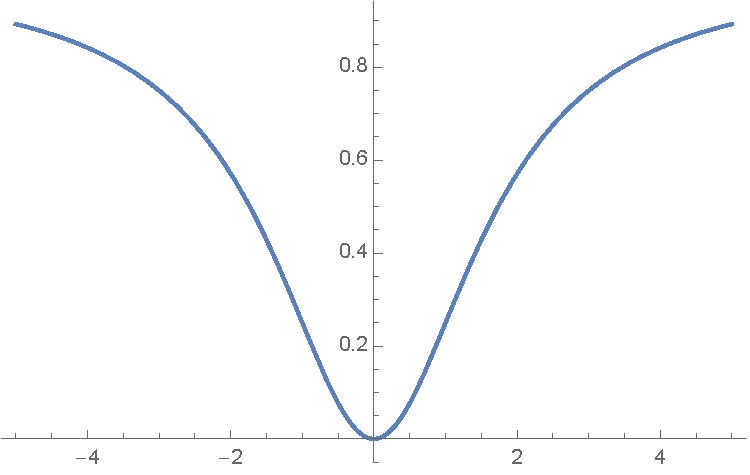
\includegraphics[scale = 0.5]{figures_1.2/ex12.pdf}
          \caption{Exercise 12}
          \label{fig:ex12}
        \end{figure}

        The slope is the reduction in spaces rented for every extra dollar in
        fee charged. 

        The y-intercept is the number of spaces he would rent if he gave them
        away for free.

        If he charges more than \$50 per space, nobody will come.

      \item[13] 
        \begin{figure}[H]
          \centering
          \includegraphics[scale = 0.5]{figures_1.2/ex13.pdf}
          \caption{Exercise 13}
          \label{fig:ex13}
        \end{figure}

        \begin{parts}
          
          \part See Figure \ref{fig:ex13}

          \part 
            The slope is the number of Fahrenheit degrees that correspond to one
            Celsius degree. 

            The F-intercept is the Fahrenheit value for 0 Celsius degrees.
            $\unit[32\dg]{F} = \unit[0\dg]{C}$

        \end{parts}

      \item[14]
        \begin{figure}[H]
          \centering
          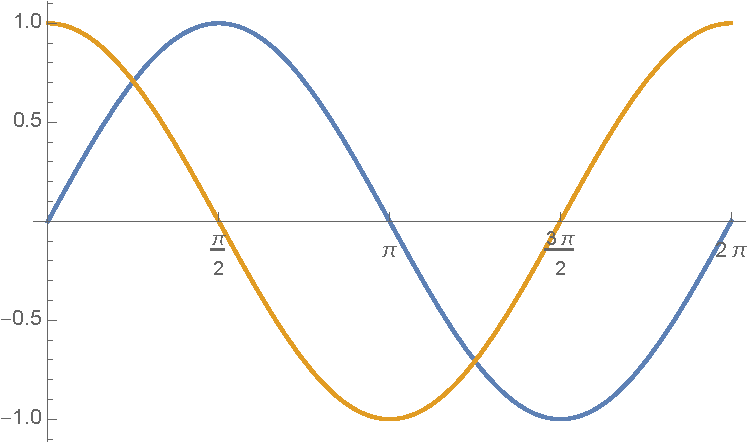
\includegraphics[scale = 0.5]{figures_1.2/ex14.pdf}
          \caption{Exercise 14}
          \label{fig:ex14}
        \end{figure}

        \begin{enumerate}[(a)]
          \item If Jason driving at a constant speed and travels 40 miles in 50
            minutes, his speed is: \[ s = \unit[48]{mi/hr} \]

            With the speed in mph, the distance traveled in terms of the time
            is:
            \[
              d(t) = 48t 
            \]

          \item See Figure \ref{fig:ex14}

          \item The slope is his speed.

        \end{enumerate}

      \item[16]
        Find the slope:
        \[
          m = \frac{4800 - 2200}{300 - 200} = \unit[13]{dollars/chair}
        \]

        Use one of the points to find the y-intercept:
        \begin{align*}
          2200 & = 100 \cdot 13 + b \\
          b    & = \unit[900]{chairs} \\
        \end{align*}

        The equation is:
        \[
          y = 13 x + 900
        \]

        \begin{itemize*}
          \item $x$ is the number of chairs produced
          \item $y$ is the cost to produce $x$ chairs
          \item $\unit[13]{dollars/chair}$ is the incremental cost to produce
            one additional chair
          \item \$900 is the cost to pay the rent and keep the factory open,
            even if you aren't producing any chairs.
        \end{itemize*}

      \item[18]
        \begin{figure}[H]
          \centering
          \includegraphics[scale = 0.5]{figures_1.2/ex18.pdf}
          \caption{Exercise 18}
          \label{fig:ex18}
        \end{figure}

        \begin{enumerate}[(a)]
          \item Use the two points to find the equation for the line:
            \begin{align*}
              380 &= 480 m + b \\
              460 &= 800 m + b \\
              \\
              c(x) &= 0.25 x + 260 \\
            \end{align*}

          \item $c(1500) = 635$

          \item See Figure \ref{fig:ex18}. The slope is the incremental cost of
            driving an additional mile.

          \item The y-intercept (\$260) is the cost of having the car, even if
            you never drive it. This is probably the fixed cost monthly of
            insurance and car payment.

          \item Part of the cost is fixed (insurance and car payment) and the
            rest of it (gas and maintenance) depends linearly on how much you
            drive.
        \end{enumerate}
        
      \item 
    \end{description}

    \subsection{Section 1.3}
    \begin{description}
      \item[1]
        \begin{enumerate}[(a)]
          \item $g(x) = f(x) + 3$
          \item $g(x) = f(x) - 3$
          \item $g(x) = f(x - 3)$
          \item $g(x) = f(x + 3)$
          \item $g(x) = f(-x)$
          \item $g(x) = -f(x)$
          \item $g(x) = 3f(x)$
          \item $g(x) = \frac{f(x)}{3}$
        \end{enumerate}

      \item[3]
        \begin{enumerate}[(a)]
          \item 3---shift right 4
          \item 1---shift up 3
          \item 4---scale vertically by 1/3
          \item 5---reflect around y-axis and shift left 4
          \item 2---scale vertically by 2 and shift left 6 
        \end{enumerate}

      \item[6]
        \begin{align*}
          g(x) & = 2 f(x - 2) \\
               & = 2 \sqrt{3(x - 2) - (x - 2)^2} \\
               & = 2 \sqrt{-x^2 + 7x - 10} \\
        \end{align*}

      \item[7]
        \begin{align*}
          g(x) & = -1 - f(x + 4) \\
               & = -1 -\sqrt{3 (x+4)-(x+4)^2} \\
               & = -1 -\sqrt{-x^2-5 x-4} \\
        \end{align*}

      \item[9] 
        \begin{figure}[H]
          \centering
          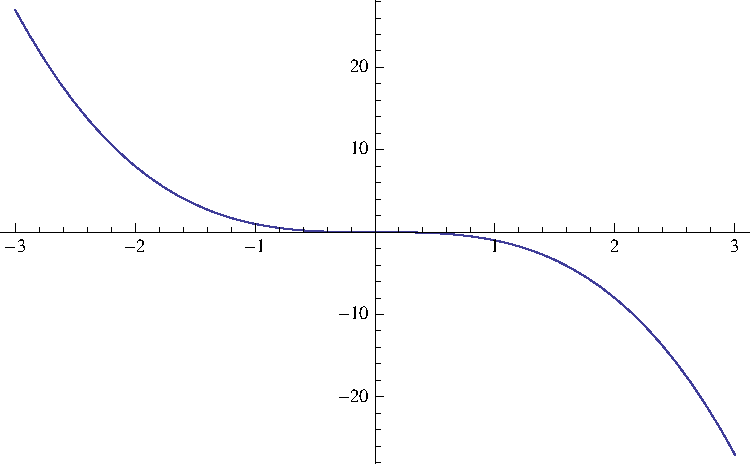
\includegraphics[scale = 0.5]{figures_1.3/ex09.pdf}
          \caption{Exercise 9}
          \label{fig:ex09}
        \end{figure}

      \item[10] 
        \begin{figure}[H]
          \centering
          \includegraphics[scale = 0.5]{figures_1.3/ex10.pdf}
          \caption{Exercise 10}
          \label{fig:ex10}
        \end{figure}

      \item[11] 
        \begin{figure}[H]
          \centering
          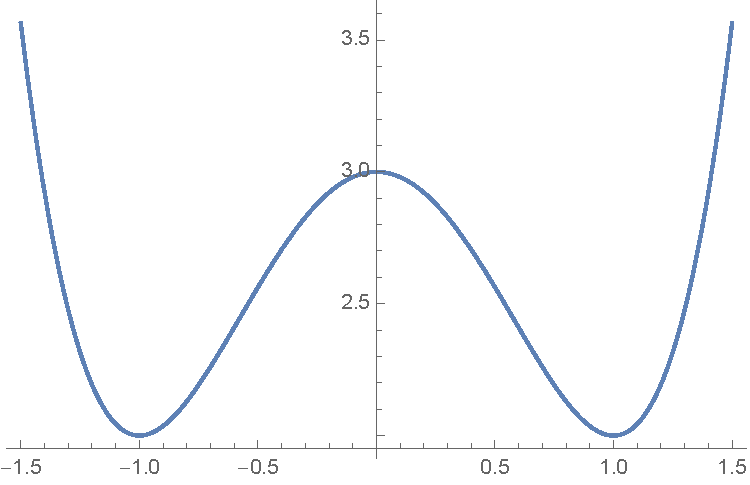
\includegraphics[scale = 0.5]{figures_1.3/ex11.pdf}
          \caption{Exercise 11}
          \label{fig:ex11}
        \end{figure}

      \item[16] 
        \begin{figure}[H]
          \centering
          \includegraphics[scale = 0.5]{figures_1.3/ex16.pdf}
          \caption{Exercise 16}
          \label{fig:ex16}
        \end{figure}

      \item[17] 
        \begin{figure}[H]
          \centering
          \includegraphics[scale = 0.5]{figures_1.3/ex17.pdf}
          \caption{Exercise 17}
          \label{fig:ex17}
        \end{figure}

      \item[31]
        \begin{align*}
          (f \circ g)(x) &= 4x^2 + 4x \\
          (g \circ f)(x) &= 2x^2 - 1 \\
          (f \circ f)(x) &= x^4 - 2x^2 \\
          (g \circ g)(x) &= 4x + 3 \\
        \end{align*}

      \item[33]
        \begin{align*}
          (f \circ g)(x) &= 1 - 3 \cos{x} \\
          (g \circ f)(x) &= \cos{ (1 - 3x) } \\
          (f \circ f)(x) &= 9x - 2 \\
          (g \circ g)(x) &= \cos { (\cos { x }) } \\
        \end{align*}

      \item[36]
        \begin{align*}
          (f \circ g)(x) &= \frac{\sin (2 x) }{\sin (2 x) +1} \\
          (g \circ f)(x) &= \sin \left( \frac{ 2x }{x+1} \right) \\
          (f \circ f)(x) &= \frac{x}{2x + 1} \\
          (g \circ g)(x) &= \sin ( 2 \sin 2x) \\
        \end{align*}

      \item[37]
        \[
          (f \circ g \circ h)(x) = 2x - 1 \\
        \]
  
      \item[38]
        \[
          (f \circ g \circ h)(x) = 2 x^2-4 x+1 \\
        \]
  
      \item[41]
        \begin{align*}
          f(x) &= x^{10} \\
          g(x) &= x^2 + 1 \\
        \end{align*}

      \item[42]
        \begin{align*}
          f(x) &= \sin x \\
          g(x) &= \sqrt{x} \\
        \end{align*}

      \item[43]
        \begin{align*}
          f(x) &= \frac{1}{1 + x} \\
          g(x) &= \sqrt[3]{x} \\
        \end{align*}

      \item[44]
        \begin{align*}
          f(x) &= \sqrt[3]{x} \\
          g(x) &= \frac{1}{1 + x} \\
        \end{align*}

      \item[45]
        \begin{align*}
          f(x) &= \sqrt{x} \\
          g(x) &= \cos x \\
        \end{align*}

      \item[46]
        \begin{align*}
          f(x) &= \frac{1}{1 + x} \\
          g(x) &= \tan x \\
        \end{align*}

      \item[47]
        \begin{align*}
          h(x) &= x^2 \\
          g(x) &= 3^x \\
          f(x) &= 1 - x \\
        \end{align*}

      \item[53]
        \begin{enumerate}[(a)]
          \item $r(t) = 60t$

          \item $A(t) = 60t$
            \begin{align*}
              A(r)      & = \pi r^2 \\
              A \circ r & = \pi (60t)^2 \\
                        & = \pi 3600 t^2 \\
            \end{align*}
        \end{enumerate}

      \item[59]
        \begin{align*}
          f \circ g & = m_1 (m_2 x + b_2) + b_1 \\
                    & = m_1 m_2 x + m_1 b_2 + b_1 \\
        \end{align*}

        This is a linear function with slope $m_1 m_2$

      \item[60]
        \begin{align*}
          A \circ A & = 1.04^2 x \\
          A \circ A \circ A & = 1.04^3 x \\
          A \circ A \circ A \circ A & = 1.04^4 x \\
        \end{align*}

        For n copies: $f(x) = 1.04^n x$

    \end{description}

  \else
    \vspace{11 cm}
    \begin{quote}
      \begin{em}
        You can't sing up on freedom, but you can swing up on some freedom.
        Power in defense of freedom is greater than power in behalf of tyranny
        and oppression.
      \end{em}
    \end{quote}
    \hspace{1 cm} --Malcolm X
  \fi

\end{document}

